\section{Unity Editor Interface}

\begin{learningoutcomes}
\item Mengenal semua panel utama Unity Editor
\item Memahami fungsi setiap panel
\item Mampu mengatur layout editor
\item Mampu melakukan navigasi dasar di Unity Editor
\end{learningoutcomes}

\subsection{Panel Utama Unity Editor}

\begin{figure}[ht]
    \centering
    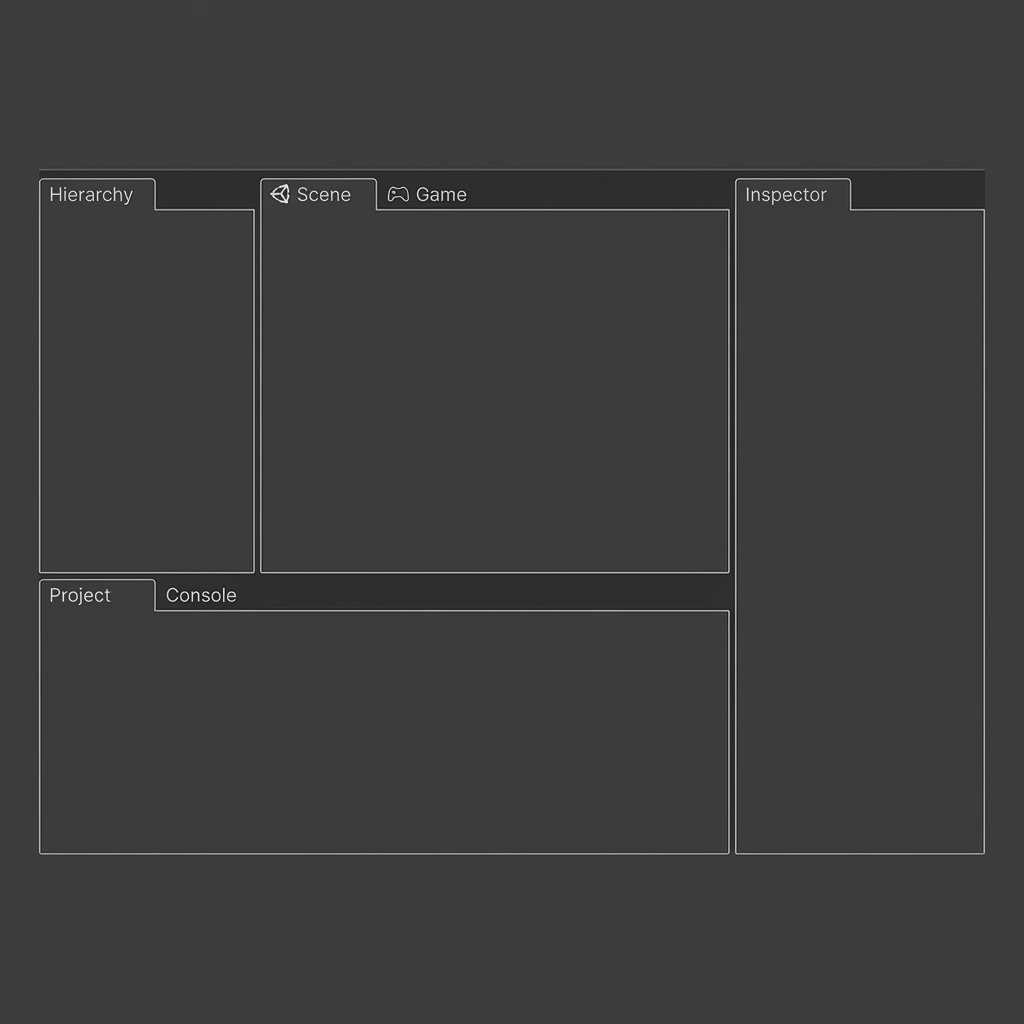
\includegraphics[width=\textwidth]{figures/unity_editor.png}
    \caption{Layout Standar Unity Editor}
    \label{fig:unity_editor}
\end{figure}

\subsubsection{Scene View}
Area untuk mengedit dan mengatur scene. Navigasi: Pan (Q), Rotate (E), Scale (R), Move (W). Gizmos untuk manipulasi objek.

\subsubsection{Game View}
Preview bagaimana game akan terlihat saat dimainkan. Aspect ratio dan resolution testing, Play mode preview.

\subsubsection{Hierarchy}
Menampilkan semua GameObject dalam scene aktif. Struktur parent-child, drag-and-drop untuk mengatur hierarchy.

\subsubsection{Inspector}
Menampilkan properti GameObject atau asset yang dipilih: Component properties, Transform values, Script variables.

\subsubsection{Project}
File browser untuk semua assets dalam project. Folder structure, asset preview, search dan filter.

\subsubsection{Console}
Menampilkan log, warning, dan error. Debug messages, error tracking.

\subsection{Shortcuts Penting}

\textbf{Ctrl/Cmd + S}: Save scene. \textbf{Ctrl/Cmd + Shift + N}: New GameObject. \textbf{F}: Focus pada objek terpilih. \textbf{Space}: Play/Pause. \textbf{Ctrl/Cmd + Shift + C}: Clear Console.
